\documentclass[12pt, a4paper, simple]{eskdtext}

\usepackage{env}
\usepackage{_sty/gpi_lstlisting}
\usepackage{hyperref}
\usepackage{_sty/gpi_table_of_content}

% Код
\def \gpiDocTypeNum {81}
\def \gpiDocVer {00}
\def \gpiCode {\gpiLetterI\gpieLetterII\gpiLetterIII.\gpiStudentGroupName\gpiStudentGroupNum.\gpiStudentCard.0\gpiDocNum~\gpiDocTypeNum~\gpiDocVer}

\def \gpiDocTopic {\gpiFIObig\/C}

% Графа 1 (наименование изделия/документа)
\ESKDcolumnI {\ESKDfontIII \gpiTopic \\ \gpiDocTopic}

% Графа 2 (обозначение документа)
\ESKDsignature {\gpiCode}

% Графа 4 (литералы)
\ESKDcolumnIVfI {\gpiLetterI}
\ESKDcolumnIVfII {\gpieLetterII}
\ESKDcolumnIVfIII {\gpiLetterIII}

% Графа 9 (наименование или различительный индекс предприятия) задает команда
\ESKDcolumnIX {\gpiDepartment}

% Графа 11 (фамилии лиц, подписывающих документ) задают команды
\ESKDcolumnXIfI {\gpiStudentSurname}
\ESKDcolumnXIfII {\gpiTeacherSurname}
\ESKDcolumnXIfV {\gpiTeacherSurname}

\begin{document}
    \begin{ESKDtitlePage}
        \hspace{0pt}\\
        \vfill
        \begin{center}
            \textbf{\ESKDfontV \gpiTopic \\ \gpiDocTopic}
        \end{center}
        \vfill
        \hspace{0pt}\\
    \end{ESKDtitlePage}
    
    \tableofcontents                                
    \thispagestyle{empty} % удаляет нумерацию страниц, которую создает библиотека
    \newpage

    \section{Краткое функциональное описание системы}

Система обеспечивает первичный ввод типизированных документов бухгалтерского учета
(операция, сумма, базовые аналитика по операции).
С последующей разноской (контировкой) данного документа в регистрационный журнал (РЖ). 

Далее из РЖ формируется книга счетов (КС),
которая служит основанием для формирования балансовой отчетности (БО).

Данная система обеспечивает минимальный комплект БО:
\begin{itemize}
    \item оборотно-сальдовая ведомость за период... по счету...;
    \item балансовая ведомость за период... по счету...;
    \item журнал-ордер за период... по счету... .
\end{itemize}


При формировании первичных документов используются картотеки справочного характера (справочники):
\begin{itemize}
    \item Определение первичных документов;
    \item Типовые хозяйственные операции (ТХО).
\end{itemize}

\newpage

    \section{Материалы предварительного проектирования системы}
\subsection{Функциональная схема обработки данных}

\begin{figure}[!htb]
    \centering
    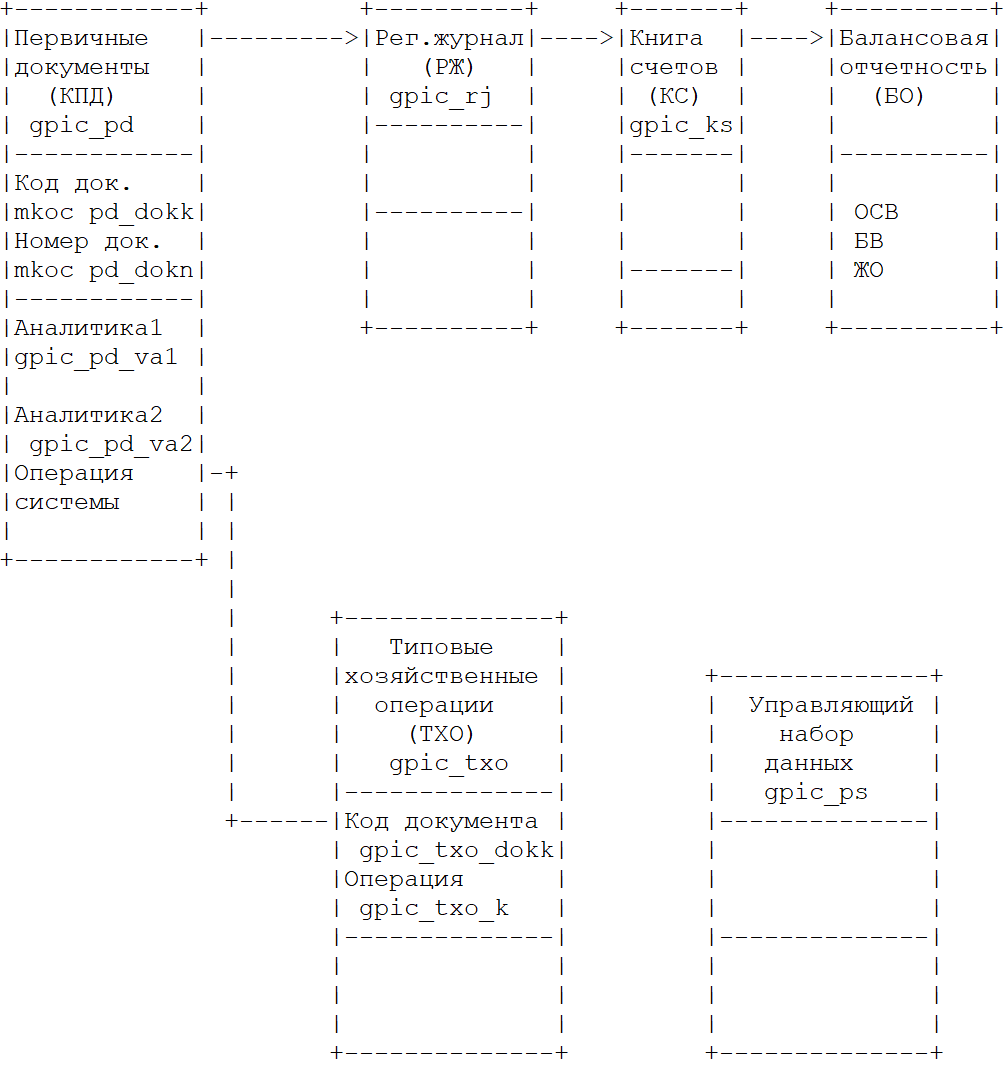
\includegraphics[width=15cm]
        {_assets/gpic_part2.png}
    \caption{Функциональная схема обработки данных}
    \label{fig:gpic_part2}
\end{figure}

\subsection{Описание картотек}

Картотеки:

\begin{itemize}
    \item Первичные документы gpic\_pd;
    \item Регистрационный журнал (РЖ) gpic\_rj;
    \item Книга счетов (КС) gpic\_ks;
    \item Типовые хозяйственные операции (ТХО) gpic\_txo.
\end{itemize}

\begin{table}[h!]
    \centering
    \scriptsize
    \caption{Первичные документы gpic\_pd}
    \begin{tabular}{|l|l|l|} 

\hline
\textbf{Реквизит}           &\textbf{Обозначение}   &\textbf{Тип и значность}   \\ \hline
код документа < --- opd     &gpic\_pd\_dokk         &c7                         \\ \hline
номер документа             &gpic\_pd\_dokn         &n4                         \\ \hline
дата документа              &gpic\_pd\_dokd         &n12                        \\ \hline
типовая операция < --- txo  &gpic\_pd\_to           &c10                        \\ \hline
дебет *txo                  &gpic\_pd\_db           &n4                         \\ \hline
дебет наименование *txo     &gpic\_pd\_dbn          &c10                        \\ \hline
кредит *txo                 &gpic\_pd\_kr           &n4                         \\ \hline
кредит наименование *txo    &gpic\_pd\_krn          &c10                        \\ \hline
сумма                       &gpic\_pd\_rub          &n4                         \\ \hline

    \end{tabular}
\end{table}

\begin{table}[h!]
    \centering
    \scriptsize
    \caption{Регистрационный журнал (РЖ) gpic\_rj}
    \begin{tabular}{|l|l|l|} 

\hline
\textbf{Реквизит}               &\textbf{Обозначение}   &\textbf{Тип и значность}   \\ \hline
дата операции                   &gpic\_rj\_data         &n12                        \\ \hline
код оправдательного документа   &gpic\_rj\_dokk         &c7                         \\ \hline
номер документа                 &gpic\_rj\_dokn         &n14                        \\ \hline
дата документа                  &gpic\_rj\_dokd         &n12                        \\ \hline
содержание операции             &gpic\_rj\_to           &c10                        \\ \hline
дебет, счет                     &gpic\_rj\_db           &n4                         \\ \hline
дебет, наименование             &gpic\_rj\_dbn          &c10                        \\ \hline
кредит, счет                    &gpic\_rj\_kr           &n4                         \\ \hline
кредит наименование             &gpic\_rj\_krn          &c10                        \\ \hline
сумма                           &gpic\_rj\_rub          &n4                         \\ \hline

    \end{tabular}
\end{table}

\begin{table}[h!]
    \centering
    \scriptsize
    \caption{Книга счетов(КС) gpic\_ks}
    \begin{tabular}{|l|l|l|} 

\hline
\textbf{Реквизит}               &\textbf{Обозначение}   &\textbf{Тип и значность}   \\ \hline
дата операции                   &gpic\_ks\_data         &n12                        \\ \hline
код оправдательного документа   &gpic\_ks\_dokk         &c7                         \\ \hline
номер документа                 &gpic\_ks\_dokn         &n4                         \\ \hline
дата документа                  &gpic\_ks\_dokd         &n12                        \\ \hline
операции                        &gpic\_ks\_to           &c10                        \\ \hline
счет                            &gpic\_ks\_s            &n4                         \\ \hline
счёт наименование               &gpic\_ks\_sn           &c10                        \\ \hline
кор. счёт                       &gpic\_ks\_ks           &n4                         \\ \hline
кор. счет наименование          &gpic\_ks\_ksn          &c10                        \\ \hline
сумма дб                        &gpic\_ks\_rubdb        &n4                         \\ \hline
сумма кр                        &gpic\_ks\_rubkr        &n4                         \\ \hline

    \end{tabular}
\end{table}

\begin{table}[h!]
    \centering
    \scriptsize
    \caption{Книга счетов(КС) gpic\_txo}
    \begin{tabular}{|l|l|l|} 

\hline
\textbf{Реквизит}               &\textbf{Обозначение}   &\textbf{Тип и значность}   \\ \hline
код документа < --- opd         &gpic\_txo\_dokk        &c7                         \\ \hline
код типовой операции            &gpic\_txo\_k           &c10                        \\ \hline
дебет, счёт < --- ps\_1         &gpic\_txo\_db          &n4                         \\ \hline
дебет, наименование * ps\_1     &gpic\_txo\_dbn         &c10                        \\ \hline
кредит < --- ps\_2              &gpic\_txo\_kr          &n4                         \\ \hline
кредит, наименование * ps\_2    &gpic\_txo\_krn         &c10                        \\ \hline

    \end{tabular}
\end{table}

\newpage

\subsection{Описание работ}

\begin{table}[h!p]
    \centering
    \scriptsize
    \caption{Описание работ}
    \begin{tabular}{|p{8cm}|p{8cm}|} 

% = = = = = = = = = =

\hline

% = = = = = = = = = =

\textbf{Группа работ}
&
\textbf{Работы}
\\ \hline

% = = = = = = = = = =

Формирование и разноска первичных документов \par
\hspace{0pt} \par
\textbf{gpic\_Документы}
&
- gpic\_Ввод текущей даты \par
- gpic\_Ввод и разноска первичных документов(ПД)
\\ \hline

% = = = = = = = = = =

Работа с регистрационным журналом \par
\hspace{0pt} \par
\textbf{gpic\_РЖ}
&
- gpic\_Просмотр РЖ \par
- gpic\_Формирование КС из РЖ \par
- gpic\_Просмотр КС
\\ \hline

% = = = = = = = = = =

Формирование балансовой отчетности \par
\hspace{0pt} \par
\textbf{gpic\_БО}
&
- gpic\_Опеделение отчетных форм \par
- gpic\_ОСВ \par
- gpic\_БВ \par
- gpic\_Ж-О
\\ \hline

% = = = = = = = = = =

Сопровождение картотек-справочников \par
\hspace{0pt} \par
\textbf{gpic\_Картотеки}
&
- gpic\_Типовые хозяйственные операции(ТХО) \par
- gpic\_Настройка АРМа
\\ \hline

% = = = = = = = = = =

Ведение архивов \par
\hspace{0pt} \par
\textbf{gpic\_Архивы}
&
- gpic\_Копия \par
- gpic\_Восстановление
\\ \hline

% = = = = = = = = = =

Выход из системы \par
\hspace{0pt} \par
\textbf{gpic\_Выход}
&
- gpic\_Выход
\\ \hline

% = = = = = = = = = =

    \end{tabular}
\end{table}

\newpage

    \section{Эксплуатационное описание системы}
\subsection{Функциональная схема обработки данных с использованием инструментальной среды}
\subsection{Описание картотек с использованием инструментальной среды}
\subsection{Скриншоты меню}
\subsection{Скриншоты карточек}
\subsection{Образцы первичных документов}
\subsection{Образцы печатных форм}
\newpage

    \section{Электронная версия разработанной системы}
\newpage

\end{document}
